\chapter{Intégration du projet dans le cadre de cours}
\thispagestyle{fancy}

On souhaite intégrer notre projet dans le cadre de plusieurs cours enseignés par Jean Rouat.
\smallbreak
\begin{itemize}
	\item \textbf{Cours gradué de techniques avancées en traitement des signaux.} Ce cours enseigne les différentes méthodes de représentation d'un signal dans le domaine spectral (transformée de Fourier, transformation en ondelettes, etc.), ainsi que les outils de filtrage spectral (Analyse en composantes principales, analyse en composantes indépendantes). Cours enseigné à la session d'automne. 
	\smallbreak
	\item\textbf{APP d'intelligence probabiliste}. Ce cours s'intéresse aux différentes méthodes de classification, et notamment les méthodes paramétriques (Bayesiennes) et non paramétriques (k-moyen, SVM, etc.). Cours enseigné à la session d'automne.
	\smallbreak
	\item \textbf{Cours de neurosciences computationnelles}. Ce cours enseigne les principes de base de la physiologie des réseaux neuronaux et leurs modélisations. Il offre également une vision d'ensemble des différents domaines d'application. Cours enseigné à la session d'hiver.
\end{itemize} 

On propose donc différents travaux pratiques permettant aux étudiants de mettre en application leurs connaissances acquises au cours de la matière.

\section{Choix des outils mathématiques d'apprentissage}

Afin d'intégrer notre liaison cerveau-ordinateur dans les différents cours, on souhaite exporter les données traitées dans OpenViBE vers un environnement de développement mathématique, afin que les élèves puissent travailler sur les signaux. Trois environnements s'offrent à nous : 
\smallbreak
\begin{itemize}
	\item \textbf{Matlab}. Il s'agit d'un langage de programmation haut niveau, associé à un environnement de développement portant le même nom. L'avantage de cet outil est qu'il est assez simple à appréhender et que la plupart des étudiants l'ont déjà utilisé à de nombreuses reprises. OpenViBE offre la possibilité d'exécuter du code Matlab sous son environnement et de l'utiliser dans la chaine de traitement des signaux EEG. Cela nécessite cependant d'utiliser Matlab 32 bits sur les ordinateurs des laboratoires, or ceux-ci possèdent uniquement la version 64 bits. Un autre de ses inconvénients 
	est qu'il s'agit d'un logiciel payant.  
	\smallbreak
	\item \textbf{Octave.} Octave est un langage de programmation mathématique de haut-niveau. Il a l'avantage d'être totalement gratuit. Cependant, OpenViBE ne propose aucune solution d'intégration d'Octave directement dans l'interface du logiciel.
	\smallbreak
	\item \textbf{Python.} Il s'agit d'un langage de programmation haut-niveau. OpenViBE propose une solution d'intégration de Python dans son environnement afin de l'utiliser dans la chaine de traitement des signaux. Cependant, cette intégration est complexe à mettre en place et nécessite de la part des élèves des connaissances autre que la simple maitrise du langage. 
\end{itemize}
\smallbreak
Aucun des environnement proposés ne semble être intégrable directement dans OpenViBE. On propose donc comme alternative d'exporter les données traitées sous OpenViBE vers un fichier CSV. Ce format représente des données tabulaires sous forme de valeurs séparées par des virgules. Il a donc l'avantage d'être lisible directement par l'Homme et de nombreux logiciels de traitement de données, comme Matlab ou même Excel. Nous proposons donc d'utiliser Matlab comme environnement de travail pour la réalisation des travaux pratiques.

\section{Cours de neurosciences computationnelles}

\subsection{Résumé du travail pratique proposé}

Le travail pratique que nous proposons aux étudiants dans le cadre du cours de neurosciences computationnelles correspond plus à un travail d'observation et de compréhension des différentes étapes de traitement des signaux électroencéphalographiques. On leur demande d'étudier le lien entre les connaissances physiologiques acquises lors du cours et les différents aspects techniques de l'interface cerveau-ordinateur. 

Pour cela, on fournit le scénario 4 (Figure \ref{scenario_neuro}) réalisé dans le cadre de l'expérience simple (partie \ref{Chapitre : Première exprérience simple d'interaction}). L'entrainement du classificateur et du filtre spatial CSP ayant été réalisé en amont, on demande donc aux étudiants de s'intéresser uniquement à l'exécution en temps réel de l'interface cerveau-ordinateur. Plusieurs outils de visualisation ont été intégré au scénario, afin que les étudiants puissent observer l'activité cérébrale (Figure \ref{cours_neuro}): 

\begin{itemize}
	\item \textbf{2D topographic map.} Permet d'observer l'activité cérébrale de l'individu portant le casque sur une représentation en 2 dimensions du crâne.
	\smallbreak
	\item \textbf{3D topographic map.} Permet d'observer l'activité cérébrale de l'individu portant le casque sur une représentation en 3 dimensions du crâne.
	\smallbreak
	\item \textbf{Signal display.} Permet d'observer les signaux EEG à différentes étapes de leur traitement (en sortie du casque EEG, après filtrage temporel).
	\smallbreak
	\item \textbf{Post CSP Display.} Permet d'observer les signaux et plus particulièrement la sélection des canaux (signaux de sortie des électrodes) après le filtrage spatial de type CSP.
	\smallbreak
	\item \textbf{Power spectrum display.} Permet d'observer les différents spectres des signaux après transformation en série de Fourier. 
	\smallbreak
	\item \textbf{Graz Visualisation.} Permet d'observer les résultats de l'expérience après classification des données.
\end{itemize}

\begin{figure}[h]
	\centering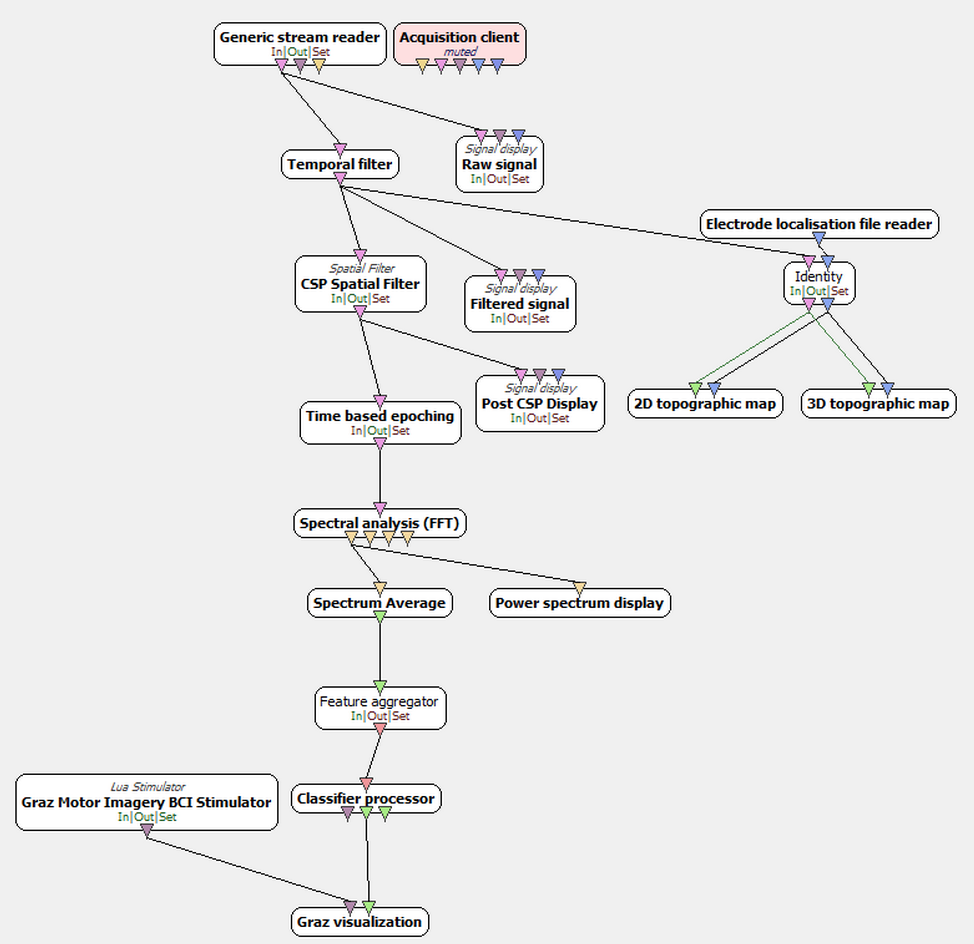
\includegraphics[height=15cm]{images/scenario_neuro.png}
	\caption[Scénario temps réel proposé dans le cadre du cours de neurosciences computationnelles.]{Scénario temps réel proposé dans le cadre du cours de neurosciences computationnelles.}
	\label{scenario_neuro}
\end{figure}

\begin{figure}[h]
	\centering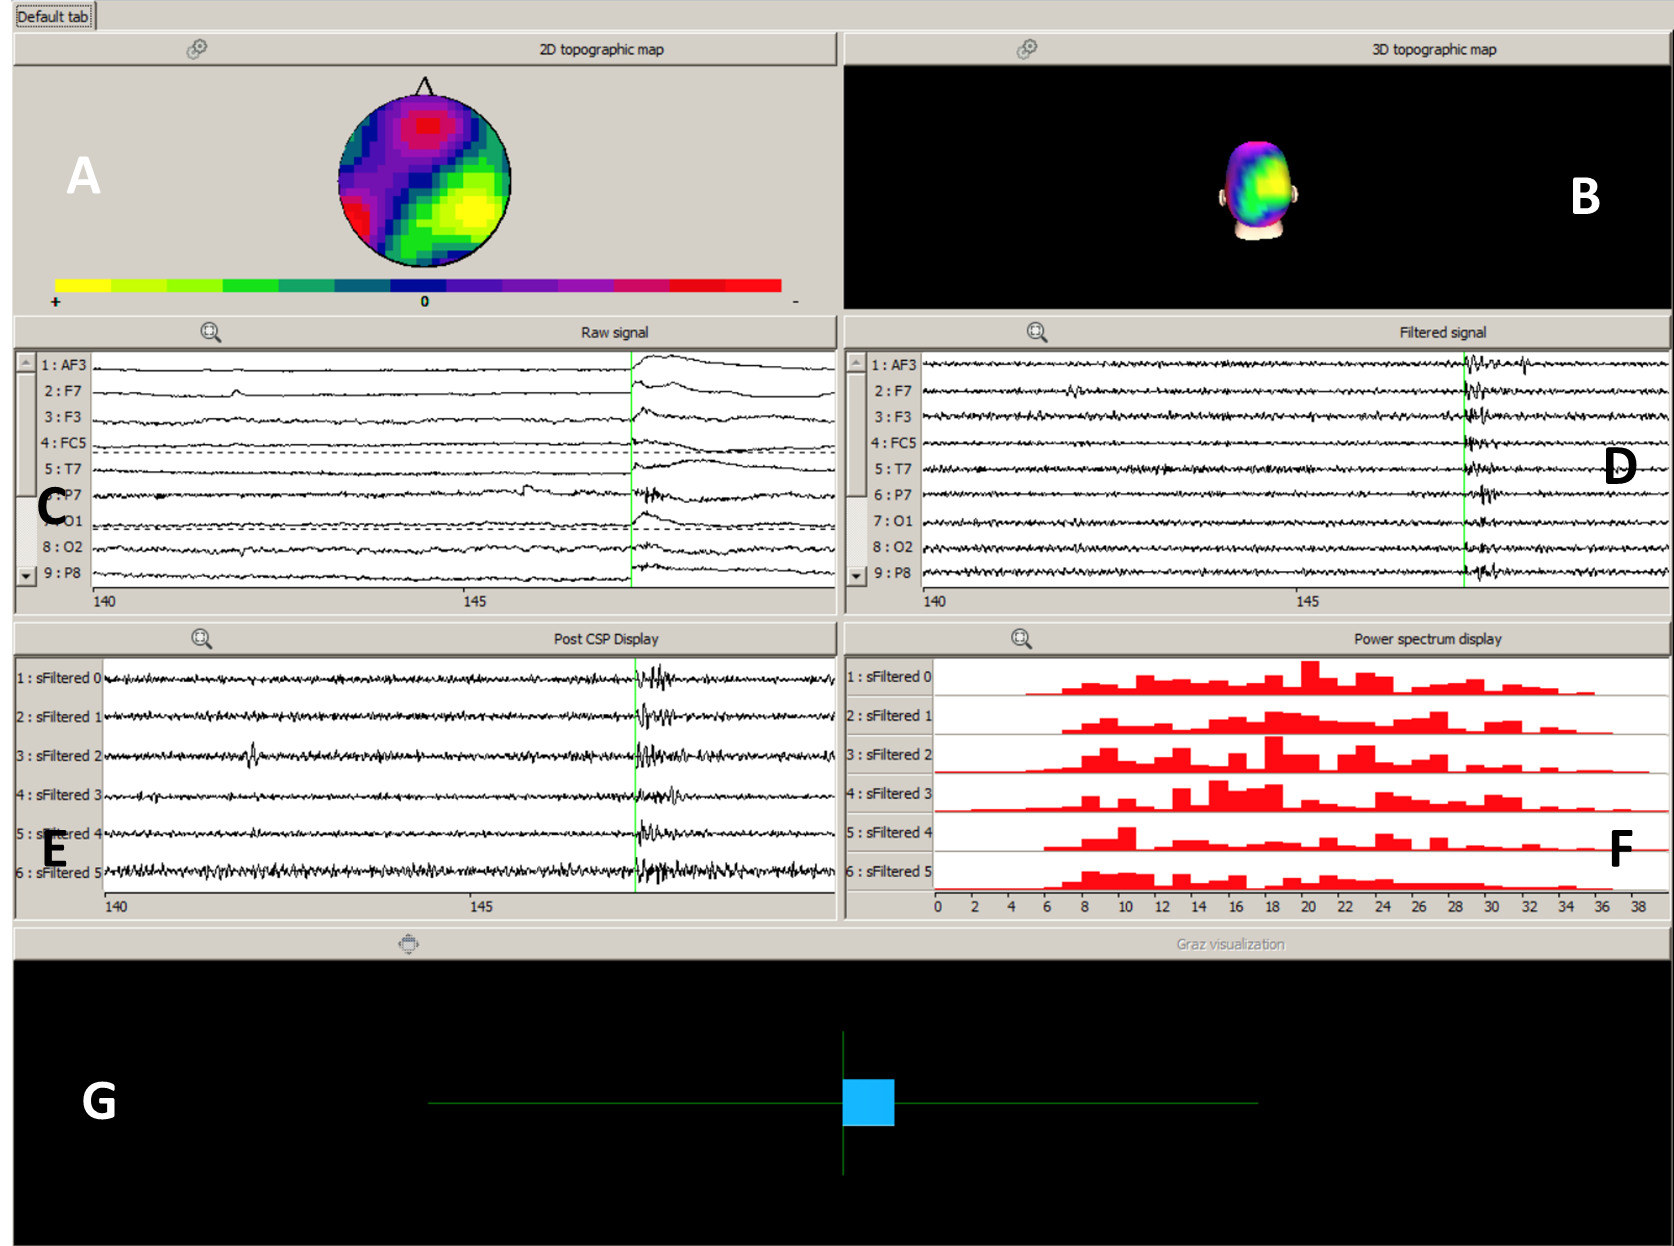
\includegraphics[height=12cm]{images/cours_neuro.png}
	\caption[Interface de visualisation proposée aux étudiants du cours de neurosciences]{Interface de visualisation proposée aux étudiants du cours de neurosciences. (A) Visualisation topographique de l'activité cérébrale en 2D. (B) Visualisation topographique de l'activité cérébrale en 3D. (C) Visualisation des signaux en sortie du casque, i.e. les signaux non traités. (D) Visualisation des signaux après filtrage temporel. (E) Visualisation des signaux après filtrage spatial CSP. (F) Visualisation des spectres fréquentiels après FFT. (G) Fenêtre de visualisation  }
	\label{cours_neuro}
\end{figure}

\subsection{Préparation du travail pratique par le professeur}

Le TP reposant uniquement sur le scénario 4, on propose ici deux approches pour la préparation du cours de neurosciences.

\subsubsection{Travail en groupe}

\begin{enumerate}
	\item Le professeur réalise en amont l'acquisition des signaux EEG (scénario 1), l'entrainement du filtre CSP (scénario 2) et l'entrainement du classificateur LDA (scénario 3).
	\smallbreak
	\item La classe ne disposant que d'un seul casque, le professeur exécutera devant l'ensemble des élèves le scénario 4 en l'utilisant grâce au bloc "Acquisition Client". Cela nécessite donc de configurer préalablement OpenViBE et le casque EPOC comme présenté en partie \ref{Chapitre : Utilisation du casque EPOC et d'OpenViBE}.
	\smallbreak
	\item  Les fichiers de configuration générés par les scénarios 2 et 3 sont utilisés pour exécuter le  scénario 4 lors du cours. Pour cela, on renseigne le chemin vers les fichiers de configuration dans les blocs "CSP spatial Filter" et "Classifier Processor".
	\smallbreak
	\item Vérifier dans le bloc "Graz Visualisation" que la case "Show instruction" est bien décochée.
\end{enumerate}

\subsubsection{Travail individuel}

\begin{enumerate}
	\item Les élèves sont dans un premier temps invités à télécharger OpenViBE.
	\smallbreak
	\item On fournit alors à l'ensemble des élèves le scénario 4, ainsi que les fichiers de configuration du filtre spatial CSP et du classificateur LDA, générés par nos soins.
	\smallbreak
	\item La classe ne disposant que d'un casque, on propose d'utiliser en entrée du scénario 4 un fichier contenant un enregistrement de signaux EEG (extension .ov), lisible avec le bloc "Generic Stream Reader". Chaque élève peut alors réaliser individuellement le travail pratique. 
	\smallbreak
	\item Vérifier dans le bloc "Graz Visualisation" que la case "Show instruction" est bien cochée, afin que l'élève puisse visualiser les consignes que l'individu avait en entrée lors de l'enregistrement. 
\end{enumerate}
  

Un sujet de travail pratique à destination des élèves a été rédigé et placé en annexe. Il contient la procédure pour réaliser la manipulation, ainsi que des questions portant sur l'interface cerveau-ordinateur. 

\section{Cours de traitement de signal avancé}

\subsection{Résumé du travail pratique proposé}

Le travail pratique que nous proposons aux étudiants du cours de traitement du signal avancé consiste à réaliser une partie de la chaine de traitement des signaux EEG de l'expérience (partie \ref*{Chapitre : Première exprérience simple d'interaction}), sous l'environnement Matlab. L'objectif est de leur permettre de mettre en application leurs connaissances (filtrage spatial, filtrage temporel, FFT). Le reste de la chaîne de traitement étant effectué sous OpenViBE, on exporte donc les données de OpenViBE vers Matlab grâce au format CSV. Une fois les signaux traités sous Matlab, on exporte à nouveaux ces données vers OpenViBE. Cette méthode de transfert entre les deux logiciels nous oblige cependant à ne pas utiliser l'interface cerveau-ordinateur en temps réel. 

\subsection{Développement de nouveaux scénarios}

Pour ce cours, nous avons implémenté trois nouveaux scénarios. Un seul sera présenté aux étudiants, les deux autres servant à la préparation du travail pratique :
\smallbreak
\begin{itemize}
	\item \textbf{Scénario d'acquisition et de filtrage temporel.} (Figure \ref{acqui2}) 
	L'objectif de ce scénario est de pouvoir récupérer les données en sortie des électrodes du casque EEG filtrées temporellement, afin d'en extraire les rythmes alpha et bêta. Son principe de fonctionnement reste le même que le scénario 1 présenté dans la partie \ref{Subsection : 6.Scénario 1}. Les signaux filtrés ainsi que les données de stimulation sont exportées dans deux fichiers au format .csv. Les données de stimulation correspondent aux stimulations visuelles envoyées à l'utilisateur lors de l'enregistrement des données EEG. Le fichier CSV contenant ces données de stimulation sera utilisé par la suite pour l'entrainement du classificateur. Le fichier CSV contenant les données EEG sera quant à lui utilisé à deux reprises, lors de l'entrainement du classificateur et lors de l'execution de la liaison cerveau-ordinateur. 
		\begin{figure}[h]
			\centering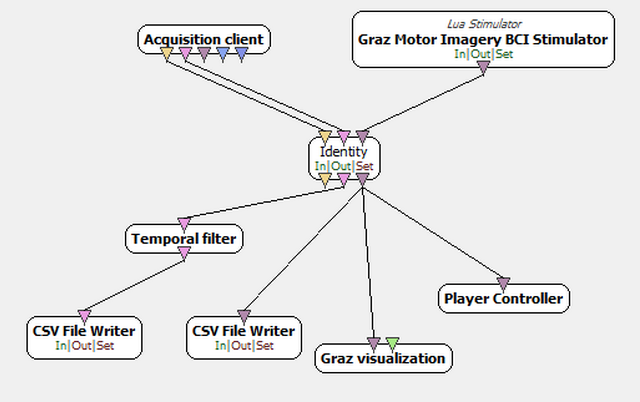
\includegraphics[height=8cm]{images/scenario_2_0.png}
			\caption{Scénario d'acquisition avec sortie au format CSV}
			\label{acqui2}
		\end{figure}
	\smallbreak
	\item \textbf{Scénario d'entrainement du classificateur}. Il permet d'entrainer le classificateur de type LDA (Figure \ref{classi2}).  Le principe de fonctionnement reste identique au scénario présenté dans la partie \ref{Subsection : 6.Scénario 3}. Le scénario nécessite à son entrée deux fichiers CSV. Le premier contient les données reçues du casque lors de la phase d'acquisition après filtrage spatial ICA ou PCA sous Matlab. Le deuxième fichier contient les données de stimulation obtenues lors de la phase d'acquisition.
			\begin{figure}[h]
				\centering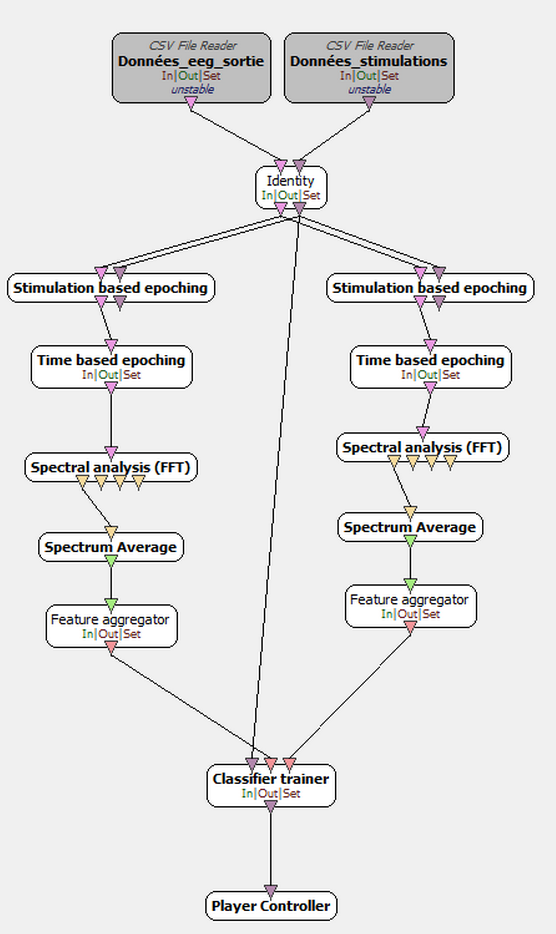
\includegraphics[height=17cm]{images/scenario_2_1.png}
				\caption{Scénario d'entrainement du classificateur à partir de fichiers .csv}
				\label{classi2}
			\end{figure}
	\smallbreak
	\item \textbf{Scénario d'exécution de l'interface cerveau-ordinateur.} Il permet d'exécuter la liaison cerveau-ordinateur (Figure \ref{obs2}). Pour cela, on utilise le fichier CSV issu du premier scénario (scénario d'acquisition) filtré spatialement avec Matlab. Le principe et la configuration du reste des blocs sont les mêmes que ceux détaillés dans la partie \ref{Subsection : 6.Scénario 4}
				\begin{figure}[h]
					\centering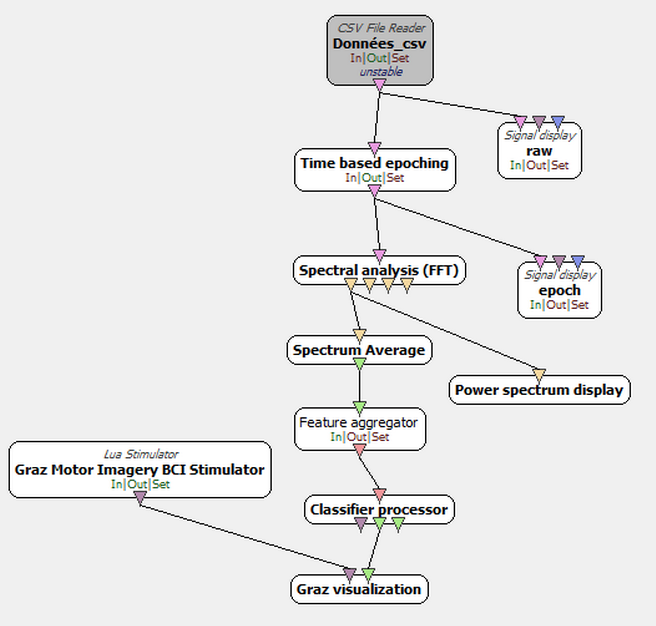
\includegraphics[height=14cm]{images/scenario_2_2.png}
					\caption{Scénario d'observation à partir de fichiers .csv issus de Matlab}
					\label{obs2}
				\end{figure}
	\smallbreak
\end{itemize}

\subsection{Fonctions Matlab et corrections}

Plusieurs fonctions Matlab ont été écrites par nos soins et sont fournies au professeur et aux élèves pour ce travail pratique :

\begin{itemize}
	\item \textbf{Une fonction de lecture pour les fichiers CSV}. Permet de lire les données EEG contenues dans un fichier de type .csv. Disponible en annexe.
	\item \textbf{Une fonction d'écriture pour les fichiers CSV}. Permet d'écrire dans un fichier .csv. Disponible en annexe.
	\item \textbf{Un sujet pour réaliser un filtrage ICA}. Contient la boucle de traitement à effectuer. La fonction permettant de faire un filtrage ICA reste à coder par les étudiants.
	\item \textbf{La correction pour réaliser un filtrage ICA}. Disponible en annexe.
	\item \textbf{Un sujet pour réaliser un filtrage PCA}. Contient la boucle de traitement à effectuer. La fonction permettant de faire un filtrage PCA reste à coder par les étudiants.
	\item \textbf{La correction pour réaliser un filtrage PCA}. Disponible en annexe.
\end{itemize}


\subsection{Préparation du travail pratique par le professeur}

Le TP reposant uniquement sur le scénario d'exécution de l'interface cerveau-ordinateur,  on propose deux approches pour la préparation du cours de neurosciences.

\subsubsection{Approche 1}

Dans cette approche, le professeur réalise en amont du TP l'acquisition des données pour l'entrainement du classificateur, l'acquisition des données pour l'exécution de l'interface cerveau-ordinateur et l'entrainement du classificateur.

\begin{enumerate}
	\item La première étape consiste à récupérer des données à partir du casque EEG et les données de stimulation. Pour cela, on utilisera le scénario d'acquisition. L'exécution du scénario génère alors deux fichiers CSV : 1 fichier "données\_entrée.csv" contenant les données EEG, 1 fichier "données\_stimulations.csv" l'autre les données de stimulation. Vérifiez dans le bloc "Graz Visualisation" que la case "Show instructions" est bien cochée.  
	\smallbreak 
	\item Le professeur est ensuite invité à exécuter le code Matlab "cours\_signal\_pca.m" ou "cours\_signal\_ica.m" afin de réaliser un filtrage spatial des données EEG. Veuillez pour cela à placer le fichier "données\_entrée.csv" généré dans l'étape précédente dans le même répertoire de travail que le code Matlab. Un fichier CSV "données\_EEG\_sortie.csv" contenant les signaux EEG filtrés est alors généré.
	\smallbreak
	\item On doit à présent entrainer le classificateur LDA. Pour cela, on utilise le scénario "entrainement du classificateur". On demande de fournir en entrée du scénario le fichier "données\_EEG\_sortie.csv" généré précédemment ainsi que le fichier "données\_stimulations.csv" généré lors de l'exécution du scénario "acquisition". L'exécution du scénario génère un fichier de configuration en sortie "Classifier.cfg".
	\smallbreak
	\item Enfin, on demande d'exécuter de nouveau le scénario d'acquisition afin d'obtenir des données EEG différentes de celles utilisées pour l'entrainement du classificateur afin d'exécuter l'interface cerveau-ordinateur. On veillera cette fois-ci à décocher la case "Show instructions" dans le bloc "Graz Visualisation" afin de ne pas être influencé par la présence des stimulations lors de l'acquisition des données. L'utilisateur est alors invité à penser à sa main gauche ou sa main droite chaque fois que le repère blanc apparait dans la fenêtre de visualisation (Celui-ci n'apparait qu'au bout de 30 secondes).
	\smallbreak
	\item Le professeur fournira à ses élèves le fichier de configuration du classificateur ("Classifier.cfg"), ainsi que le dernier fichier "données\_entrée.csv" généré. Cela permettra aux étudiants d'utiliser le scénario "execution de l'interface cerveau-ordinateur". 
\end{enumerate}


\subsubsection{Approche 2}
Dans cette approche, le professeur n'a pas besoin de réaliser un travail préparatoire en amont du TP (entrainement classificateur, acquisition de données EEG). Celui-ci fournit simplement à ses étudiants le fichier de configuration du classificateur et le fichier "données\_entrées.csv". Cela leur permettra d'utiliser le scénario "execution de l'interface cerveau-ordinateur".